% Synthetic fixture: the strokes both artifacts draw alike — a chain of
% continuing segments is one path whose interior vertices join instead of
% capping, a zero line width is the thinnest visible line rather than none,
% and a dashed chain keeps one dash pattern around its corner. Invented
% content and design.
\documentclass{article}

\pictures{ tool = none }

\fonts{ dir = "fonts", body = "Source Serif Pro" }

\title{Joined Strokes}
\author{Pat Placeholder}

\begin{document}

\maketitle

\section{A chain, a hairline, a dashed corner}

Before the strokes, a chain of segments turns its corner as one path.

\begin{center}
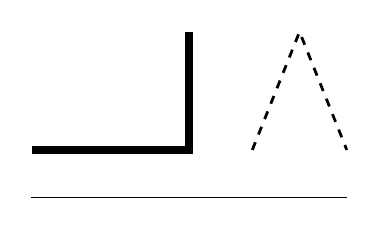
\begin{tikzpicture}
  \draw[line width=3pt] (0,0) -- (2,0) -- (2,1.5);
  \draw[line width=0pt] (0,-0.6) -- (4,-0.6);
  \draw[dashed, line width=1pt] (2.8,0) -- (3.4,1.5) -- (4,0);
\end{tikzpicture}
\end{center}

After the strokes, the prose resumes.

\end{document}
